\section{Discussion}
\subsection{CIFAR-10 dataset}
The Madry et al. attack challenge is open to two datasets: MNIST and CIFAR-10. We only choose MNIST for this work due to computational resource limitations. A fully vectorized, single attack on the MNIST dataset containing 10000 images takes between 5 minutes and 1 hour, depending on the attack complexity and the number of steps taken. Initial runs for CIFAR-10 using the same vectorized code took more than 12 hours per attack. This is largely due to two reasons: increased image size and greater neural network model complexity. Each CIFAR-10 image contains almost 4x the number of input pixels compared to MNIST. In addition, the defense model for MNIST is relatively simple; a shallow convolutional neural network model can accurately classify MNIST, resulting in relatively quick cross-entropy loss gradient calculations. However, the CIFAR-10 challenge uses a Resnet model, which significantly increases the gradient computation time per iteration.

\subsection{Attack images}
Example images that are misclassified by the defense model are shown in Figure \ref{fig:adv_example_images}. The images produced would not be incorrectly classified by humans but are clearly wrongly labeled by the classifier. In other cases not shown, some images may be difficult for even a human to classify.

\begin{figure}
    \centering
    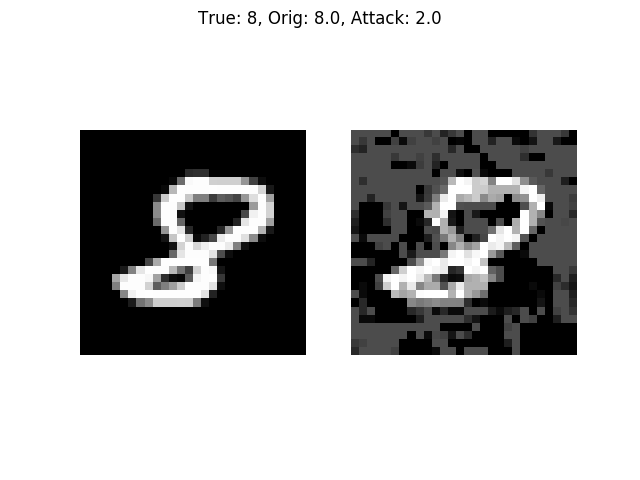
\includegraphics[width=6cm]{Report/sections/images/sample_61.png}
    \qquad
    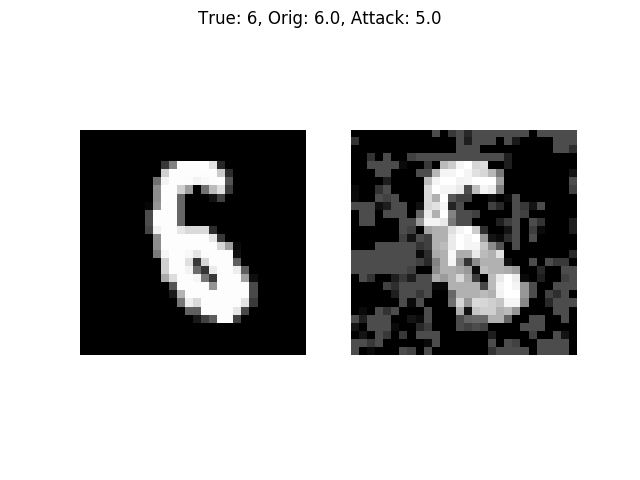
\includegraphics[width=6cm]{Report/sections/images/sample_1182.png}
    \caption{Example adversarial images generated by 'clipped-pixels' partial iterative FGSM attack}
    \label{fig:adv_example_images}
\end{figure}

\subsection{Comparison to reported baselines}
The best variation of partial iterative FGSM attack found was the 'clipped-pixels' variant, which achieved an attack accuracy of 92.31\%. We compare our results to two types of baselines: best attack as reported by the public attack challenge and best attack that we are able to reproduce.

The best attack for the MNIST challenge is named Distributionally Adversarial Attack, which achieves a test accuracy of 88.79\%. Since our model is based off FGSM and its variants, we also compare to the best reported accuracy of a loss-gradient step method. The best accuracy reported for this type of attack is PGD on cross entropy loss, which achieves 89.62\%. These attacks clearly outperform clipped-pixels.

The results in Table \ref{tab:res_table} compare 'clipped-pixels' against baselines ran from the popular Cleverhans library. We ran a hyperparameter search for each baseline and report the best result found. The baseline hyperparameter search generally agrees with the public challenge results: PGD is the most successful attack on the MNIST dataset. We also attempted to reproduce the PGD results from the public challenge using the same originally reported hyperparameters. Unfortunately, the best accuracy we were able to produce was 92.52\%, which is significantly worse than the publicly reported best accuracy. The lack of reproducibility could be simply due to randomness since the PGD implementation uses a random initial perturbation of each image before performing the gradient steps. Our reproduced results indicate that clipped-pixels is competitive with PGD and that further exploration of partial iterative FGSM variants could produce promising results.

\begin{figure}
    \centering
    % 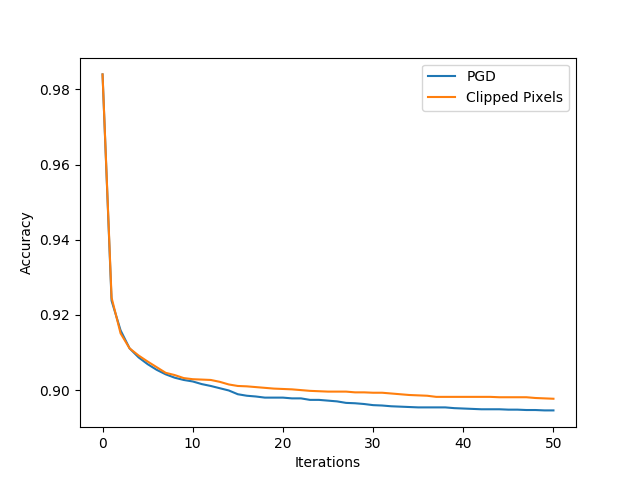
\includegraphics[width=6cm]{Report/sections/images/PGD_CLIP_trainingplot.png}
    
\includegraphics[width=6cm]{Report/sections/images/pikachu.jpg}
    \caption{PGD vs Clipped Pixels, iteratively attacking the model.}
    \label{fig:PGDvCLIP}
\end{figure}

To further explore PGD reproducibility, we attempted to understand the "random restarts" condition by as performing multiple attacks. At each attack, we only perturb images that the prior evaluation step correctly classified, and keep the adversarial images that were successfully misclassified. Since we only reperturb classified images, this strictly decreases the final accuracy. By performing these steps, we reach a final PGD accuracy of \textbf{89.46\%}, which is very similar to the reported 89.62\%. When we use this method for Clipped Pixels we get an accuracy of \TODO{fill in number here \textbf{10.00\%}}.A plot of this process showing the improvement of accuracy over iterations is shown in Figure \ref{fig:PGDvCLIP}. We find that there is marginal improvement after 50 iterations. The original paper is not clear how to reproduce their result, but we believe this is a reasonable interpretation, even though it significantly increases the runtime.

\subsection{Why do our attacks work?}
Since the top gradients method selects pixels to update at each iteration, there exists some distribution of pixel updates over the entire attack. We plot this pixel update frequency in a heatmap, where the heatmap indicates how many times a pixel was updated during the attack on that image. An example heatmap is shown in Figure \ref{fig:heatmap}. The heatmap provides some insight into which pixels dominate the loss gradient over the entire attack. In the figure, we see an image that is successfully attacked, and while the attacked image still appears to be a 9, the heatmap indicates the attack's pixel preference to push it towards a 5 by focusing on the right half of the image. 

\begin{figure}
    \centering
    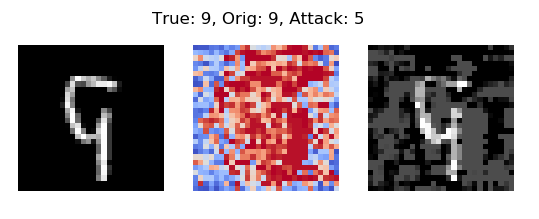
\includegraphics{Report/sections/images/heatmap.png}
    \caption{Pixel update frequency heatmap for a successful attack.}
    \label{fig:heatmap}
\end{figure}

\subsection{Hyperparameter search}
We performed an initial hyperparameter search on each developed model by exponentially increasing every hyperparameter, allowing us to quickly find useful parameter limits. We then perform a fine-grained hyperparameter search for each model and report the best test accuracies found. An example output of the search for the Top Gradients attack is shown in Figure \ref{fig:hyperparam_search}.

\begin{figure}
    \centering
    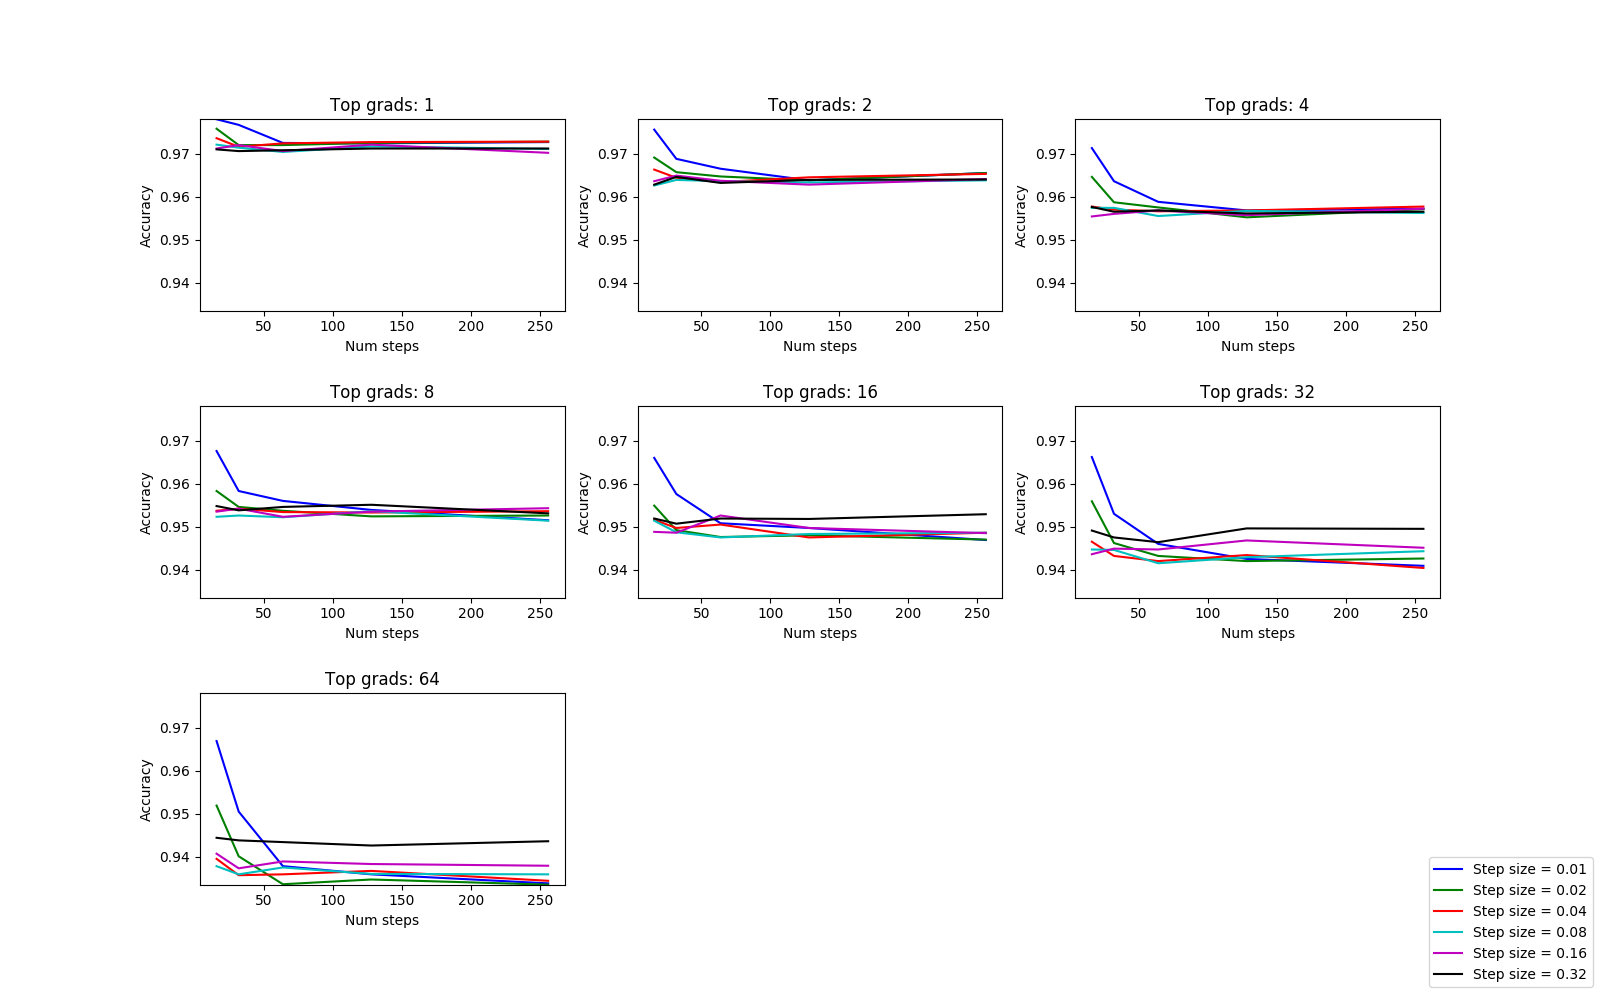
\includegraphics[width=\textwidth]{Report/sections/images/hyperparameter-search.png}
    \caption{Hyperparameter search results for Top Gradients attack. Hyperparameters include step size, number of steps, and number of top gradients selected for update.}
    \label{fig:hyperparam_search}
\end{figure}

\subsection{Future work}
The core idea of partial iterative FGSM - selectively choosing which pixels to update at each gradient step - is a promising variation of the successful iterative FGSM attack. Ideas for future work include: 

\begin{itemize}
\item Testing partial iterative FGSM attacks on CIFAR-10
\item Investigate why we could not reproduce results using the attack baselines on MNIST
\item Create new attack methods with better results than the baseline models

\end{itemize}
